%\documentclass[12pt]{article}
\documentclass[12pt]{scrartcl}
\title{ELEC 340 Assignment 3}
\nonstopmode
%\usepackage[utf-8]{inputenc}
\usepackage{graphicx} % Required for including pictures
\usepackage[figurename=Figure]{caption}
\usepackage{float}    % For tables and other floats
\usepackage{verbatim} % For comments and other
\usepackage{amsmath}  % For math
\usepackage{amssymb}  % For more math
\usepackage{fullpage} % Set margins and place page numbers at bottom center
\usepackage{paralist} % paragraph spacing
\usepackage{listings} % For source code
\usepackage{subfig}   % For subfigures
%\usepackage{physics}  % for simplified dv, and 
\usepackage{enumitem} % useful for itemization
\usepackage{siunitx}  % standardization of si units

\usepackage{tikz,bm} % Useful for drawing plots
%\usepackage{tikz-3dplot}
\usepackage{circuitikz}

%%% Colours used in field vectors and propagation direction
\definecolor{mycolor}{rgb}{1,0.2,0.3}
\definecolor{brightgreen}{rgb}{0.4, 1.0, 0.0}
\definecolor{britishracinggreen}{rgb}{0.0, 0.26, 0.15}
\definecolor{cadmiumgreen}{rgb}{0.0, 0.42, 0.24}
\definecolor{ceruleanblue}{rgb}{0.16, 0.32, 0.75}
\definecolor{darkelectricblue}{rgb}{0.33, 0.41, 0.47}
\definecolor{darkpowderblue}{rgb}{0.0, 0.2, 0.6}
\definecolor{darktangerine}{rgb}{1.0, 0.66, 0.07}
\definecolor{emerald}{rgb}{0.31, 0.78, 0.47}
\definecolor{palatinatepurple}{rgb}{0.41, 0.16, 0.38}
\definecolor{pastelviolet}{rgb}{0.8, 0.6, 0.79}
\begin{document}

\begin{center}
	\hrule
	\vspace{.4cm}
	{\textbf { \large ELEC 340 --- Applied Electromagnetics and Photonics}}
\end{center}
{\textbf{Name:}\ David Li \hspace{\fill} \textbf{Due Date:} January 25 2018, 11:30 AM   \\
{ \textbf{Student Number:}} \ V00818631 \hspace{\fill} \textbf{Assignment:} Number 3 \\
	\hrule

\paragraph*{Problem 1} %\hfill \newline
 Given that the electric field in free space is:

\[
E(R, \theta,t) = \hat{\mathbf{\theta}} \frac{2}{R} \sin(\theta) \cos(6 \pi \times 10^9 t - 2 \pi R) \ \si{m \volt / \meter}
\]
 where $R$ and $\theta$ are the radial and polar variable in the spherical coordinate system. Find:

\begin{enumerate}[label=(\alph*)]
\item The phasor representation of the given electric field vector. \newline 
$\tilde{\mathbf{E}}(R,\theta)=\hat{\mathbf{\theta}}E_\theta = \hat{\mathbf{\theta}}\frac{2}{R}\sin(\theta)e^{-j2\pi R} \si{m \volt / \meter}$
\item The phasor representation of the associated magnetic field vector. \newline 
\begin{align*}
& \nabla \times \tilde{\mathbf{E}} = j \omega \mu  \tilde{\mathbf{H}} \\
& \tilde{\mathbf{H}}=\frac{1}{j \omega \mu }  \nabla \times \tilde{\mathbf{E}}
\end{align*}

\begin{align*}
 \nabla \times \tilde{\mathbf{E}} = \frac{1}{R \sin{\theta}}\left( \frac{\partial}{\partial \theta}(E_\phi sin(\theta)) - 
\frac{\partial E_\theta}{\partial \phi}\right) \hat{\mathbf{R}} & +  \frac{1}{R} \left(\frac{1}{\sin(\theta)}\frac{\partial E_R}{\partial \phi} - \frac{\partial}{\partial R}(R E_{\phi})\right)\hat{\mathbf{\theta}} \\
& + \frac{1}{R}\left(\frac{\partial}{\partial R}(R E_\theta) - \frac{\partial E_R}{\partial \theta}\right)\hat{\mathbf{\phi}}
\end{align*}
Since $\tilde{\mathbf{E}}$ only has non-zero values in the  $\hat{\mathbf{\phi}}$ direction.
\begin{align*}
& \nabla \times \tilde{\mathbf{E}} = \frac{1}{r \sin{\theta}}\left( \ 
-\frac{\partial E_\theta}{\partial \phi}\right) \hat{\mathbf{R}}-\frac{1}{R}\frac{\partial}{\partial R} (RE_\theta) \hat{\mathbf{\phi}}= - \left(\frac{1}{R \sin{\theta}}\left( 
\frac{\partial E_\theta}{\partial \phi}\right) \hat{\mathbf{R}}+\frac{1}{R}\frac{\partial}{\partial R} (RE_\theta)\hat{\mathbf{\phi}} \right)
\end{align*}
\begin{align*}
 \tilde{\mathbf{H}} & =-\frac{1}{j \omega \mu }  \nabla \times \tilde{\mathbf{E}}= \frac{-1}{j \omega \mu} \hat{\mathbf{\phi}} \frac{0.002}{R} \sin{\theta} \frac{\partial}{\partial R} (e^{-j 2\pi R}) \\
 & =\hat{\mathbf{\phi}} \frac{2\pi}{j6 \pi \times 10^9 \times 4 \pi \times 10^{-7}}\frac{0.002}{R} \sin(\theta) e^{-j2 \pi R} \\
 & = \hat{\mathbf{\phi}} \frac{5.30516477 \times 10^{-7}}{R} \sin(\theta) e^{-j 2 \pi R - \pi / 2} \ \left( \si{\ampere / \meter} \right) \\
 & = \hat{\mathbf{\phi}} \ \frac{53}{R} sin(\theta) e^{-j 2 \pi R - \pi / 2} \ (\si{\mu \ampere / \meter})
\end{align*}
\item The time-domain representation of the magnetic field you obtained in (b). 
\begin{align*}
& = \hat{\mathbf{\phi}} \ \frac{53}{R} \sin(\theta) \cos(6\pi \times 10^{9} t -2 \pi R - \pi / 2) \ (\si{\mu \ampere / \meter})
\end{align*}
\end{enumerate}
\paragraph*{Problem 2}
The electric field intensity of a 5-MHz linearly polarized uniform plane wave traveling in free space in 10 V/m. The electric field is polarized in the +z direction at t = 0 and the wave in propagating in the -y direction. Find:
\begin{enumerate}[label=(\alph*)]
\item The angular frequency and wave number, and intrinsic wave impedance. \newline 
Since the plane wave is traveling in free space, $\mu = \mu_0$ and $\epsilon=\epsilon_0$.
% See https://www.wolframalpha.com/input/?i=sqrt(4+%5Ctimes+pi+%5Ctimes+10%5E%7B-7%7D+%5Ctimes++8.854187+%5Ctimes+10%5E%7B-12%7D)
\begin{align*}
& \omega = 2\pi f = 10 \pi \si{M \hertz} \quad k=\omega\sqrt{\mu \epsilon} = 10 \pi \ \times 10^6 \times 3.335641 \times 10^{-9} = 0.0334 \pi \  \si{\radian / \meter}
\end{align*}
The intrinsic impedance of a lossless medium is defined as:
\begin{align}
\eta = \frac{\omega \mu}{k}=\frac{\omega \mu}{\omega \sqrt{\mu \epsilon}}=\frac{\mu}{\epsilon} \qquad (\si{\ohm})
\end{align}
Since free space is being used: $\eta = \eta_0= 120 \pi \Omega$
\item The field vectors phasor, i.e. $\mathbf{\tilde{E}}$ and $\mathbf{\tilde{H}}$ \newline 
\begin{align*}
& \tilde{\mathbf{E}}= - \mathbf{\hat{y}}E_0=  - \mathbf{\hat{y}}10 e^{-j 0.0334 \pi  z} \si{\volt / \meter} \\
& \nabla \times \tilde{\mathbf{E}} = \left(\frac{\partial E_z}{\partial y} - \frac{\partial E_y}{\partial z} \right) \mathbf{\hat{x}} + \left(\frac{\partial E_x}{\partial z} - \frac{\partial E_z}{\partial x} \right) \mathbf{\hat{y}}
+\left(\frac{\partial E_y}{\partial x} - \frac{\partial E_x}{\partial y} \right) \mathbf{\hat{z}}\\
& \tilde{\mathbf{H}}=\frac{1}{j \omega \mu }  \nabla \times \tilde{\mathbf{E}} = - \frac{1}{j \omega \mu } \frac{\partial E_y}{\partial z}\mathbf{\hat{x}} = \frac{10(0.0334 \pi) e^{-j 0.0334 \pi  z} \mathbf{\hat{x}}}{j \times 2\pi \times 10\times 10^6\times 4 \pi \times 10^{-7}} \\
& \quad =
%https://www.wolframalpha.com/input/?i=10*0.033356%2F4
\mathbf{\hat{x}} \ \frac{0.08339}{2\pi} e^{-j 0.0334 \pi  z - \pi / 2} \ \si{\ampere / \meter}
\end{align*}
\item
\begin{align*}
&  \mathbf{E} = -\hat{\mathbf{y}} 10 \cos(2\pi 10 \times 10^6 t -0.0334 \pi z)  \ \si{\volt / \meter} \\
&  \mathbf{H} = \ \ \mathbf{\hat{x}} \ 0.0132719 \cos(2\pi 10 \times 10^6 t -0.0334 \pi z - \pi /2 )   \ \si{\ampere / \meter}
\end{align*}

\newpage
\item Draw a diagram to illustrate the field vectors and propagation direction.
% \begin{center}
%   \begin{tikzpicture}[x={(-10:1cm)},y={(90:1cm)},z={(210:1cm)}]
%     % Axes
%     \draw (-1,0,0) node[above] {$x$} -- (5,0,0);
%     \draw (0,0,0) -- (0,2,0) node[above] {$y$};
%     \draw (0,0,0) -- (0,0,2) node[left] {$z$};
%     % Propagation
%     \draw[->,ultra thick] (5,0,0) -- node[above] {$c$} (6,0,0);
%     % Waves
%     \draw[thick] plot[domain=0:4.5,samples=200] (\x,{cos(deg(pi*\x))},0);
%     \draw[gray,thick] plot[domain=0:4.5,samples=200] (\x,0,{cos(deg(pi*\x))});
%     % Arrows
%     \foreach \x in {0.1,0.3,...,4.4} {
%       \draw[->,help lines] (\x,0,0) -- (\x,{cos(deg(pi*\x))},0);
%       \draw[->,help lines] (\x,0,0) -- (\x,0,{cos(deg(pi*\x))});
%     }
%     % Labels
%     \node[above right] at (0,1,0) {$\bm{E}=10\frac{V}{m}$};
%     \node[below] at (0,0,1) {$\bm{B}$};
%   \end{tikzpicture}
% \end{center}

%% lazy approach changing labels around

%\begin{center}
\centerline{
  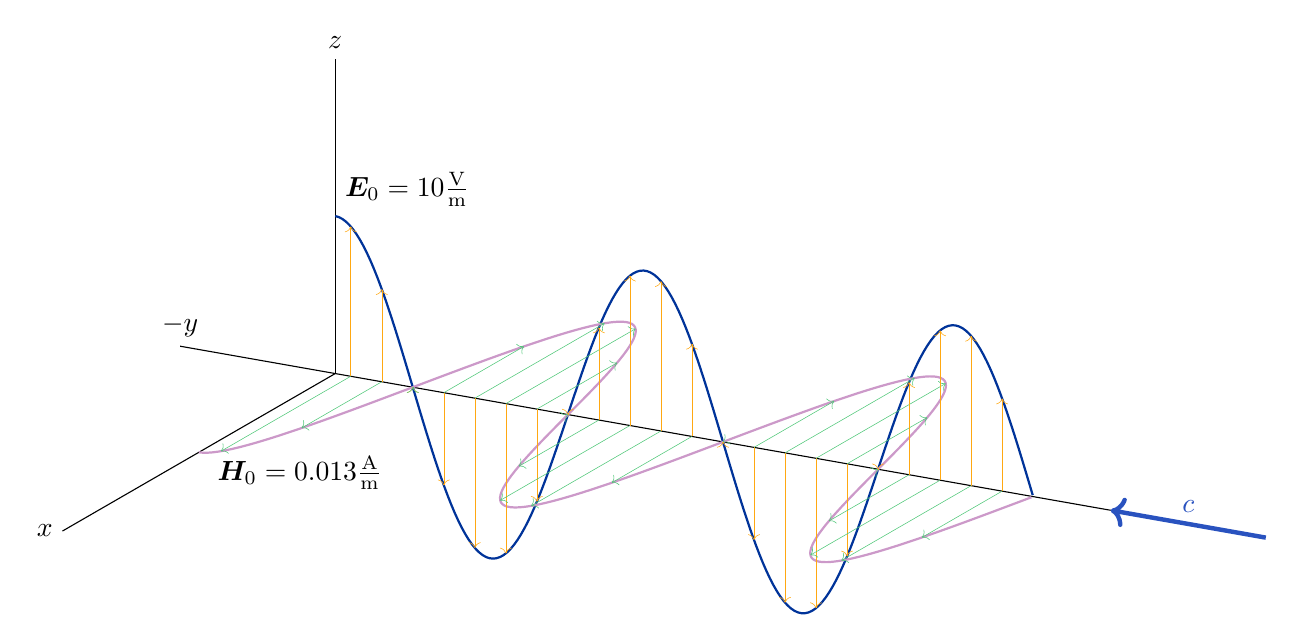
\begin{tikzpicture}[x={(-10:1cm)},y={(90:1cm)},z={(210:1cm)},scale=2]
    % Axes
    \draw (-1,0,0) node[above] {$-y$} -- (5,0,0);
    \draw (0,0,0) -- (0,2,0) node[above] {$z$};
    \draw (0,0,0) -- (0,0,2) node[left] {$x$};
    % Propagation
    \draw[->,ultra thick,ceruleanblue] (6,0,0) -- node[above] {$c$} (5,0,0);
    % Waves
    \draw[thick,darkpowderblue] plot[domain=0:4.5,samples=200] (\x,{cos(deg(pi*\x))},0);
    \draw[gray,thick,pastelviolet] plot[domain=0:4.5,samples=200] (\x,0,{cos(deg(pi*\x))});
    % Arrows
    \foreach \x in {0.1,0.3,...,4.4} {
      \draw[->,help lines,darktangerine] (\x,0,0) -- (\x,{cos(deg(pi*\x))},0);
      \draw[->,help lines,emerald] (\x,0,0) -- (\x,0,{cos(deg(pi*\x))});
    }
    % Labels
    \node[above right] at (0,1,0) {$\bm{E}_0=10 \si{\frac{\volt}{\meter}}$};
    \node[below] at (0.65,0.15,1) {$\bm{H}_0=0.013\si{\frac{\ampere}{\meter}}$};
  \end{tikzpicture}}
%\end{center}
  \begin{minipage}{.5\linewidth}
    \[
      \tilde{\mathbf{H}} = \frac{\nabla \times \tilde{\mathbf{E}}}{j \omega \mu}
    \]
    \begin{tabular}{r@{${}={}$}p{.8\linewidth}}
      $E_0$ & electric field amplitude \\
      $H_0$ & magnetic field amplitude \\ %amplitude (instantaneous values) \\
      $c$ & speed of light ($3\times10^8\mathrm{m/s}$) \\
    \end{tabular}
  \end{minipage}%
  \begin{minipage}{.5\linewidth}
    \[
      c = \frac{1}{\sqrt{\mu_0 \varepsilon_0}}
    \]
    \begin{tabular}{r@{${}={}$}p{.8\linewidth}}
      $\mu_0$ & magnetic permeability in a vacuum, $\mu_0 = 1.3\times10^{-6}\,\mathrm{N/A^2}$ \\
      $\varepsilon_0$ & electric permeability in a vacuum, $\varepsilon_0 = 8.9\times10^{-12}\,\mathrm{C^2/N m^2}$ \\
    \end{tabular}
  \end{minipage}
\end{enumerate}
\paragraph*{Problem 3}
Suppose that a uniform plane wave is traveling in the +x direction in a lossless dielectric ($\mu_r=1$) with the 100 V/m electric field in the +z direction. If the wavelength is 25 cm and the velocity of propagation is $2\times 10^8 \si{\meter / \second}$. Find:
\begin{enumerate}[label=(\alph*)]
\item The relative permittivity $\epsilon_r$ and impedance $\eta$ of the medium.
% https://www.wolframalpha.com/input/?i=solve(2*10%5E8%3D+1+%2F+sqrt(8.85*10%5E(-12)*x*4*pi*10%5E(-7)*(1)))
\begin{align*}
& u_p = \frac{\omega}{k} = \frac{1}{\sqrt{\mu \epsilon}} \\
& \epsilon_r = \frac{1}{\mu_0 \mu_r \epsilon_0 u_p^2} = \frac{ \ (1)}{4 \pi \times 10 ^{-7}  \si{\henry / \meter } \  8.85 \times 10^{-12} \si{\farad / \meter} \ (2\times 10^8 \ \si{\meter / \second})^2} = 2.24795 \\
& \eta = \frac{\mu}{\epsilon} = \frac{\mu_r \mu_0}{\epsilon_r \epsilon_0} = \frac{4 \pi \times 10 ^{-7}  \ \si{\henry / \meter }}{2.24795 \times 8.85 \times 10^{-12} \  \si{\farad / \meter}} = \frac{120 \pi}{2.24795} \Omega = 53.38197 \pi \ \Omega
\end{align*}

\item The angular frequency $\omega$ and the wave number $k$.

\begin{align*}
& \text{Wave Number:} \quad k = \frac{2\pi}{\lambda} = \frac{2 \pi}{0.25 \ \si{\meter}} = 8 \pi \ \si{\radian / \meter} \\
& \omega = \mu_p \times k = 2 \times 10^8 \ \si{\meter / \second} \times 8 \pi \ \si{\radian / \meter} = 16 \pi \times 10^8 \si{\radian / \second}
\end{align*}
\item The time-domain expressions for the electric and magnetic field vectors.

\begin{align*}
& \mathbf{\tilde{E}} = \mathbf{\hat{x}} \tilde{E}_0 = 
\mathbf{\hat{x}} 100 e^{-j k z}\cos(\omega t - k z) = 
\mathbf{\hat{x}} 100 e^{-8 \pi z} \  \si{\volt / \meter} \\ 
& \nabla \times \tilde{\mathbf{E}} = \left(\frac{\partial E_z}{\partial y} - \frac{\partial E_y}{\partial z} \right) \mathbf{\hat{x}} + \left(\frac{\partial E_x}{\partial z} - \frac{\partial E_z}{\partial x} \right) \mathbf{\hat{y}}
+\left(\frac{\partial E_y}{\partial x} - \frac{\partial E_x}{\partial y} \right) \mathbf{\hat{z}}\\
& \tilde{\mathbf{H}}=\frac{1}{j \omega \mu }  \nabla \times \tilde{\mathbf{E}} 
= \frac{1}{j \omega \mu } \frac{\partial E_x}{\partial z}\mathbf{\hat{y}} = \frac{100 (-8 \pi) e^{-j 8\pi  z} \mathbf{\hat{y}}}{j \times 16\pi \times 10\times 10^8\times 4 \pi \times 10^{-7}} 
= -\mathbf{\hat{y}} \frac{1}{8 \pi} e^{-j 8\pi  z - \pi /2}
\end{align*}
\hrule
\begin{align*}
& \mathbf{E} = \mathbf{\hat{x}}E_0 = \mathbf{\hat{x}} 100 \cos(\omega t - k z) = \mathbf{\hat{x}} 100 \cos( 16 \pi \times 10^8 t - 8 \pi z) \  \si{\volt / \meter}  \\
& \mathbf{H} = -\mathbf{\hat{y}} \frac{1}{8 \pi} \cos(16 \pi \times 10^8 t - 8 \pi z - \pi /2 ) \  \si{\ampere / \meter}
\end{align*}
\item Draw a diagram to illustrate the field vectors and propagation direction.

\begin{center}
  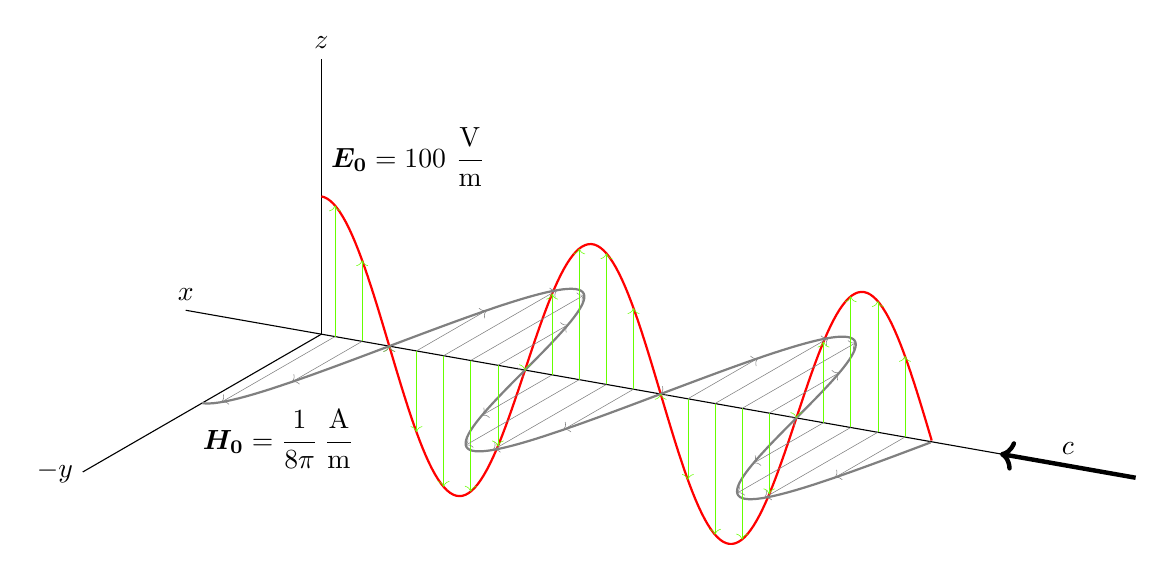
\begin{tikzpicture}[x={(-10:1.75cm)},y={(90:1.75cm)},z={(210:1.75cm)}]
    % Axes
    \draw (-1,0,0) node[above] {$x$} -- (5,0,0);
    \draw (0,0,0) -- (0,2,0) node[above] {$z$};
    \draw (0,0,0) -- (0,0,2) node[left] {$-y$};
    % Propagation
    \draw[->,ultra thick] (6,0,0) -- node[above] {$c$} (5,0,0);
    % Waves
    \draw[thick,red] plot[domain=0:4.5,samples=200] (\x,{cos(deg(pi*\x))},0);
    \draw[gray,thick] plot[domain=0:4.5,samples=200] (\x,0,{cos(deg(pi*\x))});
    % Arrows
    \foreach \x in {0.1,0.3,...,4.4} {
      \draw[->,help lines,brightgreen] (\x,0,0) -- (\x,{cos(deg(pi*\x))},0);
      \draw[->,help lines] (\x,0,0) -- (\x,0,{cos(deg(pi*\x))});
    }
    % Labels
    \node[above right] at (0,1,0) {$\bm{E_0}=100 \ \si{\cfrac{\volt}{\meter}}$};
    \node[below] at (0.55,0.15,1) {$\bm{H_0}= \cfrac{1}{8 \pi} \ \si{\cfrac{\ampere}{\meter}}$};
  \end{tikzpicture}
\end{center}
  \begin{minipage}{.5\linewidth}
    \[
      \tilde{\mathbf{H}} = \frac{\nabla \times \tilde{\mathbf{E}}}{j \omega \mu}
    \]
    \begin{tabular}{r@{${}={}$}p{.8\linewidth}}
      $E_0$ & electric field amplitude \\
      $H_0$ & magnetic field amplitude \\ %amplitude (instantaneous values) \\
      $c$ & speed of light ($3\times10^8\mathrm{m/s}$) \\
    \end{tabular}
  \end{minipage}%
  \begin{minipage}{.5\linewidth}
    \[
      c = \frac{1}{\sqrt{\mu_0 \varepsilon_0}}
    \]
    \begin{tabular}{r@{${}={}$}p{.8\linewidth}}
      $\mu_0$ & magnetic permeability in a vacuum, $\mu_0 = 1.3\times10^{-6}\,\mathrm{N/A^2}$ \\
      $\varepsilon_0$ & electric permeability in a vacuum, $\varepsilon_0 = 8.9\times10^{-12}\,\mathrm{C^2/N m^2}$ \\
    \end{tabular}
  \end{minipage}
\end{enumerate}
\end{document}
